\documentclass{article}
\usepackage{graphicx}
\usepackage{caption}
\usepackage{float}
\graphicspath{ {./images/} }

\begin{document}
\begin{figure}


Demonstration of image\\


Heaviest Bird On Earth!!!!\\

\centering
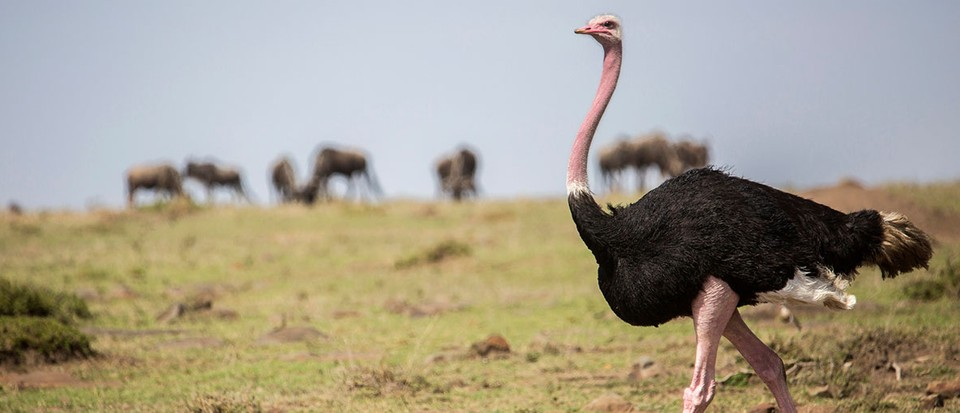
\includegraphics[width=0.8\textwidth]{ostrichh.jpg}
\caption{Ostrich}
\label{Fig:1}


Ostrich is the heaviest bird on Earth.\\


\end{figure}

Demonstration of Table\\
\begin{table}[h!]
		\begin{center}
			\caption{List of birds}
			\label{tab:table1}
			\begin{tabular}{l|c|r} % <--Alignments;1st column left ,2nd middle and 3rd right ,with vertical lines in between 
				
				\textbf{Sr. no.} & \textbf{Name} & \textbf{Avg wt(kg)}\\
				
				\hline
				1 &Common Ostrich &104\\
				2 &Somali Ostrich &90\\
				3 &Southern cassowary &45\\
				4 &Northern cassowary &44\\ %<--added row here 
			\end{tabular}
		\end{center}
	\end{table}
\end{document}
\end{document}